\chapter{Processes and concurrency}
A \emph{process} is a sequence of operations performed by a program in execution on a given set of input data. A process is a dynamic entity. It is characterized by a \textbf{Process Control Block}.

\begin{figure}[hbtp]
\centering
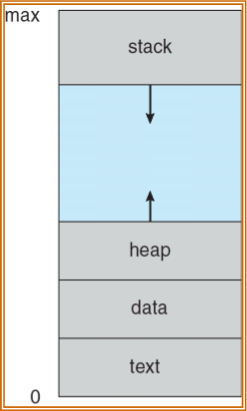
\includegraphics[scale=0.3]{images/processes_concurrency/pcb.jpg}
\caption{Process Control Block}
\end{figure}
\begin{description}
\item [Text] contains the code. This part of memory cannot be modified;
\item [Data] contains global variables;
\item [Heap] contains dynamic variables. It grows ``upward'';
\item [Stack] contains local variables and return addresses of functions. The \emph{Stack Pointer} point to the top of the stack. It grows ``downward'', so in the opposite direction to the Heap.
\end{description}

It is possible to conceptually image the \textbf{trace} of a process as a table containing values of variables and registers (stack pointer and program counter, too) at any time. In this way it is possible to know the state of the process at any instruction. In this way it is possible to perform \textbf{context switching}, the operation performed by the kernel which move the attention of the CPU from a process to a different one, restoring its state as if it was never interrupted.

Every process has a unique identifier which is called \textbf{PID}, a unique non negative integer. Although a PID is unique, UNIX reuses the numbers of terminated processes.

Library \texttt{unistd.h} contains system calls to retrieve PID:
\begin{verbatim}
pid_t getpid();    // Process ID
pid_t getppid();   // Parent process ID
uid_t getuid();    // Get the real user ID
gid_t geteuid();   // Get the effective ID
\end{verbatim}
\section{Concurrency}
Sequential processes are deterministic. \textit{Cooperating processes} have precedence constraints in order to guarantee a specific order in the process execution. Hence, processes are not more independent and some typical problem arise such as deadlock and synchronization.

\subsection{Process creation}
System call \texttt{fork} creates a new \textbf{child} process which is a perfect clone of the parent process. Those processes have the same initial value of variables and they share code and file pointers of open files (because they point to the kernel memory) but they do not share anything else (different stacks, different heaps, different data sections).

\texttt{fork()} returns two different values:
\begin{itemize}
\item The parent process receives the child PID: in this way the parent process can recognize every single child;
\item The child process receives the value 0: it does not have to receive the parent PID because it can obtain it through the system call \texttt{getppid};
\item -1 in case of error.
\end{itemize}

Library \texttt{unistd.h} contains the system call \texttt{fork()}:
\begin{verbatim}
pid_t fork(void);
\end{verbatim}

\subsection{Process termination}
When a process terminates, the kernel sends a \texttt{SIGCHLD} to its parent. Receiving a signal is an asynchronous event and the parent process may
\begin{itemize}
\item Manage the child termination:
\begin{itemize}
\item System call \texttt{wait};
\item System call \texttt{waitpid};
\item Using a signal handler for signal \texttt{SIGCHLD}.
\end{itemize}
\item Ignore the event (default behavior).
\end{itemize}

System call \texttt{wait} blocks the calling process if all its children are running (none is already terminated). \texttt{wait} will return as soon as one of its children terminates. It returns an error if the calling process has not children.

If a parent needs to wait a specific child it is better to use \texttt{waitpid}, which suspends execution of the calling process until the child, specified by \texttt{pid} argument, has changed state. By default \texttt{waitpid} waits only for terminated children.

Library \texttt{sys/wait.h} contains the system call \texttt{wait} and \texttt{waitpid}
\begin{verbatim}
pid_t wait(int *statLoc);
pid_t waitpid(pid_t pid, int *statLoc, int options);
\end{verbatim}

Parameter \texttt{statLoc} is used a return parameter which stores information about the termination of the process. There are macros to interpret its value.

\section{Move the execution}
\subsection{System call exec}
System call \texttt{exec} substitutes the process code with the executable code of another program. The new program begins its execution as usual from the main. In particular, the system call \texttt{exec} \textit{does not create a new process}, in fact it substitutes the calling process image with the image of another program and the PID does not change.

\begin{figure}[hbtp]
\centering
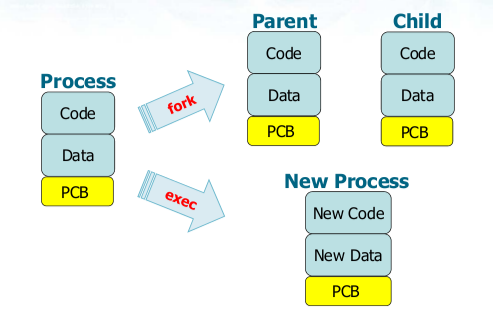
\includegraphics[scale=0.4]{images/processes_concurrency/fork_exec.png}
\caption{Different behaviors of \texttt{fork} and \texttt{exec}}
\end{figure}

There are 6 different versions of \texttt{exec} system call: \texttt{execl}, \texttt{execlp}, \texttt{execle}, \texttt{execv}, \texttt{execvp}, \texttt{execve} distinguishable by the letters:
\begin{itemize}
\item l (list): arguments are a list of strings. The last element must be a \texttt{NULL} pointer. Or equivalently, \texttt{(char *) 0}.;
\item v (vector): arguments is a vector of strings. The last element must be a \texttt{NULL} pointer. Or equivalently, \texttt{(char *) 0}.;
\item p (path): the executable filename is looked for in the directories listed in the environment variable \texttt{PATH};
\item e (environment): the last argument is an environment vector \texttt{envp[]} which defines a set of new association strings \texttt{name = value}.
\end{itemize}

Library \texttt{unistd.h} contains all the implementations of system call \texttt{exec}. They all return -1 in case of error:
\begin{verbatim}
int execl(char *path, char *arg0, ..., (char *)0);
int execlp(char *name, char *arg0, ..., (char *)0);
int execle(char *path,const char *arg0,...,char *envp[]);
int execv(char *path, char *argv[]);
int execvp(char *name, char *arg[]);
int execve(char *path, char *arg[], char *envp[]);
\end{verbatim}

\paragraph{Arguments}
\begin{itemize}
\item Pathname of the executable file: in the `p' versions the complete path is not necessary. The file must be in one of the directories listed in the environment variable \texttt{PATH}. Remember that, for security reasons, current directory is not in \texttt{PATH};
\item Its argument list: the first argument is the \textit{name} (alias) of the process (its \texttt{argv[0]}). The other arguments of the list are argument for the executable;
\item Possibly the environment vector.
\end{itemize}

\paragraph{UNIX shell skeleton}
\subparagraph{Command in foreground}
\begin{verbatim}
while(TRUE) {
    write_prompt;
    read_command(command, parameters);
    if(fork() == 0)
        /* Child: Execute command */
        execve(command, parameters);
    else
        /* Parent: Wait child */
        wait(&status);
}
\end{verbatim}

\subparagraph{Command in background (option \&)}
\begin{verbatim}
while(TRUE) {
    write_prompt;
    read_command(command, parameters);
    if(fork() == 0)
        /* Child: Execute command */
        execve(command, parameters);
    /* Parent: Continue the execution */
}
\end{verbatim}

\subsection{System call system}
System call \texttt{system} forks a shell, which executes the string command, while the parent process waits the termination of the shell command.

Library \texttt{stdlib.h} contains the system call \texttt{system}:
\begin{verbatim}
int system(const char *string);
\end{verbatim}

It returns:
\begin{itemize}
\item -1 or 127 in case of error;
\item The exit value of the shell that executed the command with the format of \texttt{waitpid}.
\end{itemize}

\section{Signals}
A \emph{signal} is a \textbf{software interrupt} (i.e.\@ asynchronous event which may occur at any time) sent to a process to notify it of an event that occurred. A signal can be used as a limited form of inter-process communication or for synchronization. The use of signals is prone to race conditions and they are difficult to manage.

\subsection{Generating a signal}
The UNIX command \texttt{KILL -SIGUSR1 4481} is used to send the \texttt{SIGUSR1} signal to process with PID 4481. Possibly signals are, \texttt{SIGUSR1}, \texttt{SIGUSR2}, \texttt{SIGALRM}, \texttt{SIGCHLD} (sent from a child process to its parent when it terminates) and \texttt{SIG\_IGN} (used to ignore a specific signal).

System call \texttt{kill} is used to send a signal \texttt{signo} to a process (or group of processes) identified by the parameter \texttt{pid}.

Library \texttt{signal.h} contains the system call \texttt{kill}:
\begin{verbatim}
int kill(pid_t pid, int signo);
\end{verbatim}

\subsection{Reacting to a signal}
A process can:
\begin{itemize}
\item ignore/discard the signal. Not possible for \texttt{SIGKILL} and \texttt{SIGSTOP} which are unmaskable;
\item execute a signal handler function.
\end{itemize}
To properly react to the asynchronous arrival of a given type of signal, a process must inform the kernel about the action that it will perform when it will receive a signal of that type. Precondition to properly handle a received signal for a process is to declare to the kernel if a signal of a given type will be ignored or caught.

System call \texttt{signal} is used to inform the kernel about the reaction, specified as an address of a function \texttt{func} to execute when a specific signal \texttt{sig} is received.

Library \texttt{signal.h} contains the system call \texttt{signal}:
\begin{verbatim}
void (*signal (int sig, void (*func)(int)))(int);
\end{verbatim}

The function \texttt{func} has this prototype: \texttt{void func(int signo)}. In this way, the same function can be used to manage different signals which can be recognized inside the signal handler.

\paragraph{Skeleton of a shell}
\subparagraph{Command in background (option \&)}
\begin{verbatim}
while(TRUE) {
    write_prompt;
    read_command(command, parameters);
    if(fork() == 0)
        /* Child: Execute command */
        execve(command, parameters);
    /* Parent: Continue the execution */
}
\end{verbatim}
Actually, this naive solution will not work because every child process becomes a zombie, given that there is no process waiting for it.

Hence, it is needed to allocate a signal handler which ignores the \texttt{SIGCHLD} generated on child termination. \texttt{signal(SIGCHLD, SIG\_IGN);}

\subsection{Issues}
If many signals of the \emph{same} type are waiting to be handled, then most UNIXs will only deliver one of them. So multiple signals are lost.

If many signals of \emph{different} types are waiting to be handled, they are not delivered in any fixed order.

It is good practice to re-allocate the handler at the end of the handler function. In fact, in some UNIX systems, the signal reaction is reset to its default action immediately after the signal has been sent.

If a signal is sent during the execution of a signal handler, the signal is lost. So, the signal handler must be short, in order to receive
``all'' signals.

\subsection{Synchronization}
The basic idea is to allocate a signal handler and to wait the signal using the system call \texttt{pause}. When a signal is received, the process will exit from the pause and will continue its execution.

Another scenario can be obtained by using the system call \texttt{alarm}. In this way, the process informs the kernel that it wants to receive a signal (\texttt{SIGALRM}) after a given amount of time \texttt{secs}. If \texttt{secs} is set to 0, the previous alarm is canceled.
It is similar to a \texttt{sleep} but it does not block the process.

Library \texttt{unistd.h} contains both the system calls \texttt{pause} and \texttt{alarm}:
\begin{verbatim}
int pause(void);
long alarm(long secs);
\end{verbatim}